\documentclass{standalone}

\usepackage{pgfplots}
\pgfplotsset{compat=1.10}   % in my packages used compat=1.15
\usepgfplotslibrary{fillbetween}
\usepackage{pgf}
\usepackage{tikz}
\usetikzlibrary{patterns,arrows,calc,decorations.pathmorphing,backgrounds, positioning,fit,petri,decorations.fractals}
\usetikzlibrary{matrix}

\usepackage[table,dvipsnames]{tudscrcolor}

\usepackage[default]{opensans}

\begin{document}
	\color{cddarkblue}
	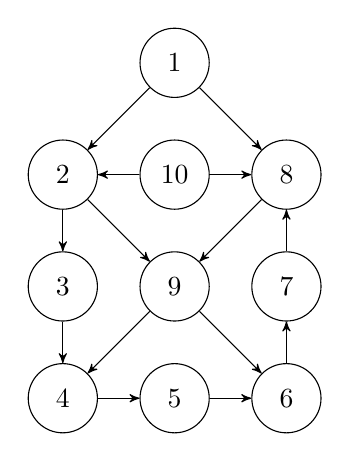
\begin{tikzpicture}[node distance=1.5em, >=stealth', every node/.style = {minimum width = 2.5em, circle, draw}]
		% Knoten
		\node (10) {10};
		\node[above=of 10] (1) {1};
		\node[left=of 10] (2) {2};
		\node[below=of 2] (3) {3};
		\node[below=of 3] (4) {4};
		\node[right=of 4] (5) {5};
		\node[right=of 5] (6) {6};
		\node[above=of 6] (7) {7};
		\node[above=of 7] (8) {8};
		\node[right=of 3] (9) {9};
	% Kanten
		\draw[->] (1) to (2);
		\draw[->] (1) to (8);
		\draw[->] (2) to (3);
		\draw[->] (2) to (9);
		\draw[->] (3) to (4);
		\draw[->] (4) to (5);
		\draw[->] (5) to (6);
		\draw[->] (6) to (7);
		\draw[->] (7) to (8);
		\draw[->] (8) to (9);
		\draw[->] (9) to (4);
		\draw[->] (9) to (6);
		\draw[->] (10) to (2);
		\draw[->] (10) to (8);
	\end{tikzpicture}
\end{document}